\subsection{きなこチーム}

\subsubsection{概要}
きなこチームは、3D-LiDARを用いた自己位置推定の信頼性向上を目的としたパッケージを開発した。
システムでは、自己位置推定にemcl2、経路計画・走行制御にNav2を採用している。
開発の背景として、人や車などの動的障害物によって自己位置推定が破綻するという課題が存在した。
この問題に対し、当初は動的障害物の影響を受けにくい2m以上の高さのスキャン点群のみを使用することで対処していた。
また、3Dマップとセンサから得られるスキャン点群を2次元に投影して処理を行っていた。
しかし、全ての点群データを単一の高さ範囲に投影すると、マップやスキャン点群の詳細な特徴が失われる。
その結果、自己位置推定の精度が著しく低下し、推定が破綻していた。
この課題を解決するため、きなこチームは新しいアプローチを導入した。
ロボットの現在位置に応じて、自己位置推定に使用するマップとスキャン点群の高さ範囲を動的に変更できるパッケージを開発した。

\subsubsection{開発したシステム}
作成したパッケージを以下に示す。

\begin{itemize}
  \item \textbf{map\_manager}
    \begin{itemize}
      \item 参照するマップを切り替えるパッケージ
      \begin{itemize}
        \item 複数の2次元マップを保持
        \item 指定した範囲にロボットが入ると、指定されたマップと指定された高さ範囲のパラメータを提供
      \end{itemize}
    \end{itemize}
  \item \textbf{pointcloud\_to\_dual\_scan}
    \begin{itemize}
      \item 3D-LiDARから2次元スキャン点群を生成するパッケージ
      \begin{itemize}
        \item 障害物回避、自己位置推定のための2つの2次元スキャン点群を生成
        \item map\_managerから高さ範囲のパラメータを受け取り、自己位置推定のためのスキャン高さ範囲を変更
      \end{itemize}
    \end{itemize}
\end{itemize}

3次元マップは事前にGLIMを使って作成した。
そのマップから実環境で見る高さと同じ高さを切り取る。
それを2次元の占有格子地図に変換する。


\subsubsection{統合}
3D-LiDARから得られたスキャン点群は、pointcloud\_to\_dual\_scanを通じて処理され、2次元スキャン点群として出力される。
このデータを用いて、nav2とemcl2が経路計画および自己位置推定を行う。
map\_managerはロボットの位置に応じて適切なマップと高さパラメータを提供し、それに基づいて自己位置推定の基盤となるマップとスキャン点群の範囲を動的に変更する。
nav2は、速度指令値を生成し、raspimouseへ送信する。
raspimouseがモータードライバを通し、モーターを動かすことでロボットが制御される。


% \begin{figure}[h]
%   \begin{center}
%     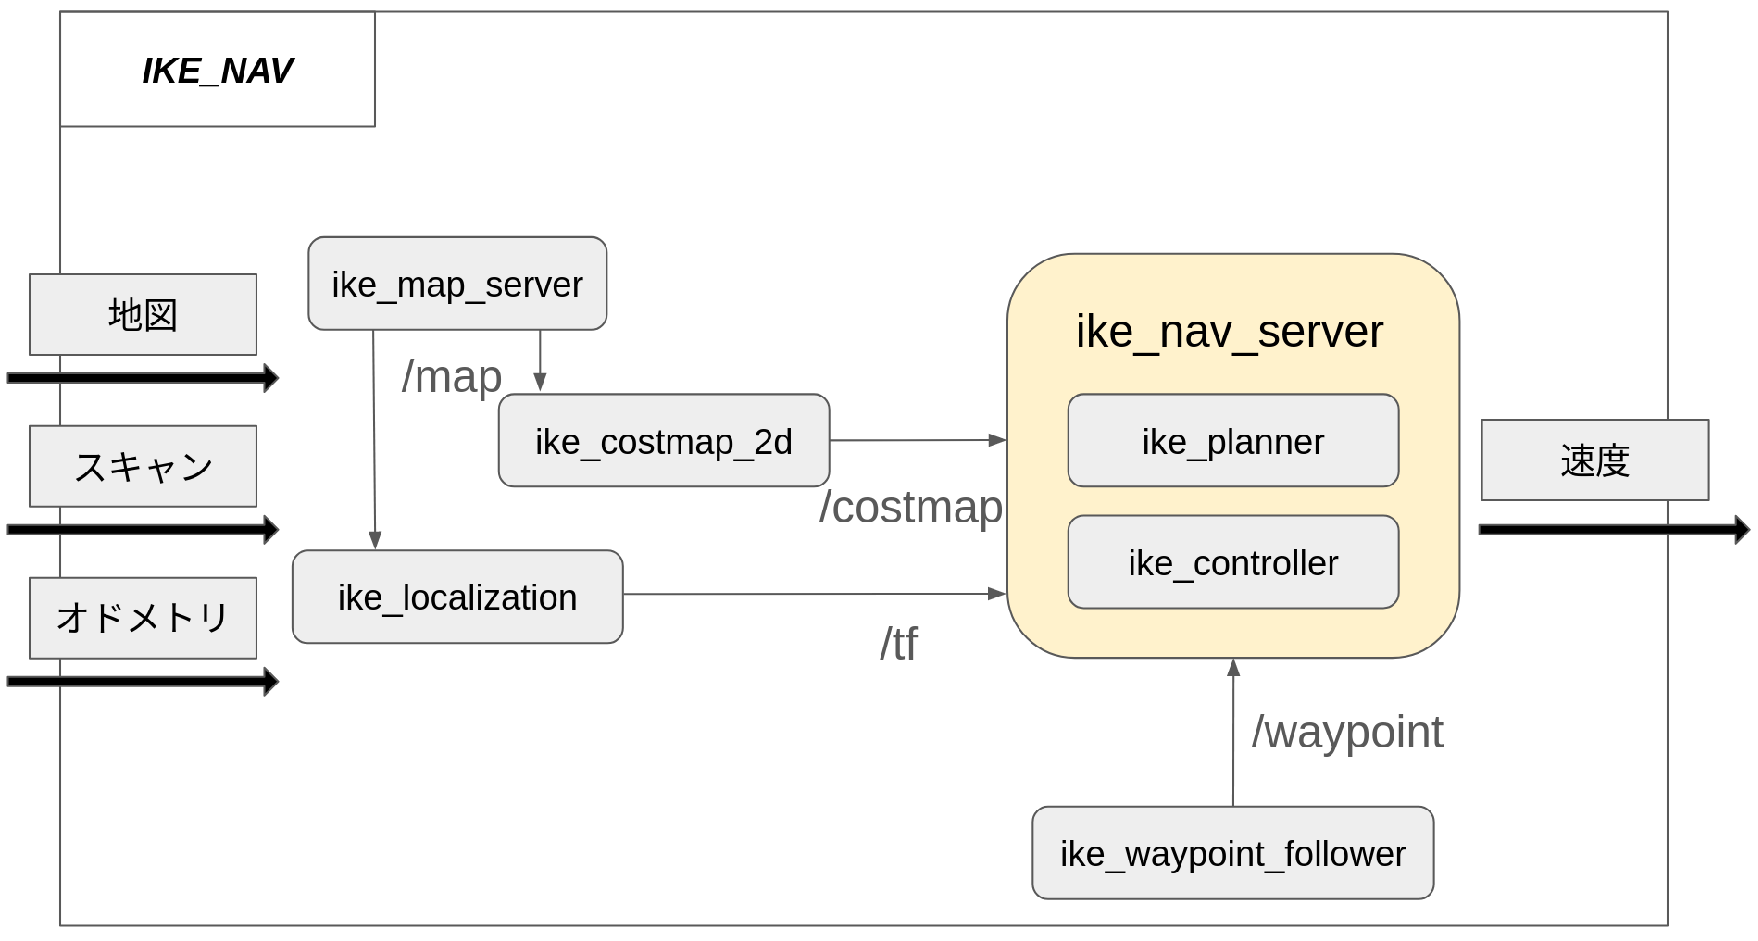
\includegraphics[width=1.0\linewidth]{figs/ike_nav.pdf}
%     \caption{ツナチームのシステム構成}
%     \label{fig:tuna_system}
%   \end{center}
% \end{figure}